\section{Обсуждение результатов}

\subsection{Результаты обучения}

В рамках данной работы был разработан автоматизированный конвейер (пайплайн), позволяющий проводить воспроизводимые эксперименты по решению проблемы фаз с помощью предложенного метода (\url{github.com/blackwood168/xrd_phase_ml}). В нем реализовано обучение и тестирование моделей, а также получение результатов на реальных массивах данных и структурах кристаллических соединений. В репозитории присутствуют маленькие наборы данных из сгенерированных и реальных структур малых органических молекул, также там представлены веса обученных в работе моделей. Воспроизводимость обучения обеспечивает фиксирование начальных значений генераторов случайных состояний.

\begin{table}[H]
\caption{Результаты обучения и эффективность дообучения моделей}
\label{doposle}
\centering
\footnotesize
\begin{tabular}{|l|l|l|l|} 
\hline
\textbf{Model} & \textbf{Metric} & \textbf{Synth} & \textbf{CSD}  \\ 
\hline
\multirow{3}{*}{UNet} 
& Before, R & 0.477 & 0.590 \\ 
& After, R  & 0.632 & 0.393 \\ 
& $\Delta$, \%       & -32.6 & 33.4  \\
\hline
\multirow{3}{*}{FFT\_UNet}
& Before, R & 0.726 & 0.646 \\ 
& After, R  & 0.619 & \textbf{0.336} \\ 
& $\Delta$, \%       & 14.7  & 48.0  \\
\hline
\multirow{3}{*}{XRD\_Transformer}
& Before, R & 0.346 & 0.581 \\ 
& After, R  & 0.615 & 0.358 \\ 
& $\Delta$, \%       & -77.9 & 38.4  \\
\hline
\end{tabular}
\end{table}

Было проведено обучение на синтетических данных и последующее дообучение на реальных. Сравнение R-фактора для моделей до и после дообучения представлено в таблице \ref{doposle}. После дообучение на реальных данных точность предсказания моделей увеличивается минимум в 1.5 раза, однако теряют в точности на синтетических данных, кроме кастомного UNet с Фурье-преобразованием. Лучшую точность имеет модель UNet\_FFT, от которой немного отстает трансформер. В сводной таблице \ref{svod} представлены значения метрик на реальных данных финальных моделей. Таким образом, UNet\_FFT занимает меньше видеопамяти, работает быстрее и достигает лучшей метрики на тестовых реальных данных.

\begin{table}[H]
\centering
\caption{Значения метрик на тестовом реальном наборе данных моделей после дообучения}
\label{svod}
\begin{tabular}{|c|c|c|c|} 
\hline
\diagbox{\textbf{Metric}}{\textbf{Model}} & \textbf{UNet} & \textbf{FFT\_UNet} & \textbf{XRD\_Transformer}  \\ 
\hline
MSE$\cdot10^{-3}$                               & 1,39      & 1,20           & 1,31                   \\ 
\hline
R                                & 0,393         & \textbf{0,336}              & 0,358                      \\
\hline
\end{tabular}
\end{table}

\subsection{Анализ моделей}

Для более глубокого понимания трансформера был проведен анализ внутренней работы модели. Особый интерес представляют карты внимания (рис. \ref{attention_maps}), которые визуализируют, как модель распределяет свое внимание при обработке дифракционных данных тестовой реальной кристаллической структуры. Механизм внимания в трансформере позволяет модели определять, какие части входных данных наиболее важны для принятия решения в каждый момент времени. В первых слоях трансформера внимание распределено равномерно и рассеянно по всей структуре данных. Это соответствует этапу сбора общего контекста, когда модель пытается получить целостное представление о кристаллической структуре. В последующих слоях внимание становится более сфокусированным и локализованным, что указывает на то, что модель научилась выделять специфические взаимосвязи между различными частями данных. Важно отметить способность модели устанавливать связи между отражениями, находящимися на значительном расстоянии друг от друга в обратном пространстве. Это критически важно для решения проблемы фаз, так как часто ключевые взаимосвязи существуют между отражениями, которые не являются ближайшими соседями. Кроме того, наблюдаются характерные диагональные паттерны внимания, которые коррелируют с известными систематическими погасаниями в кристаллографии. Можно предположить, что модель глубокого обучения без явного указания из обучающей выборки выучила механизм погасаний.

\begin{figure}[H]
    \centering
    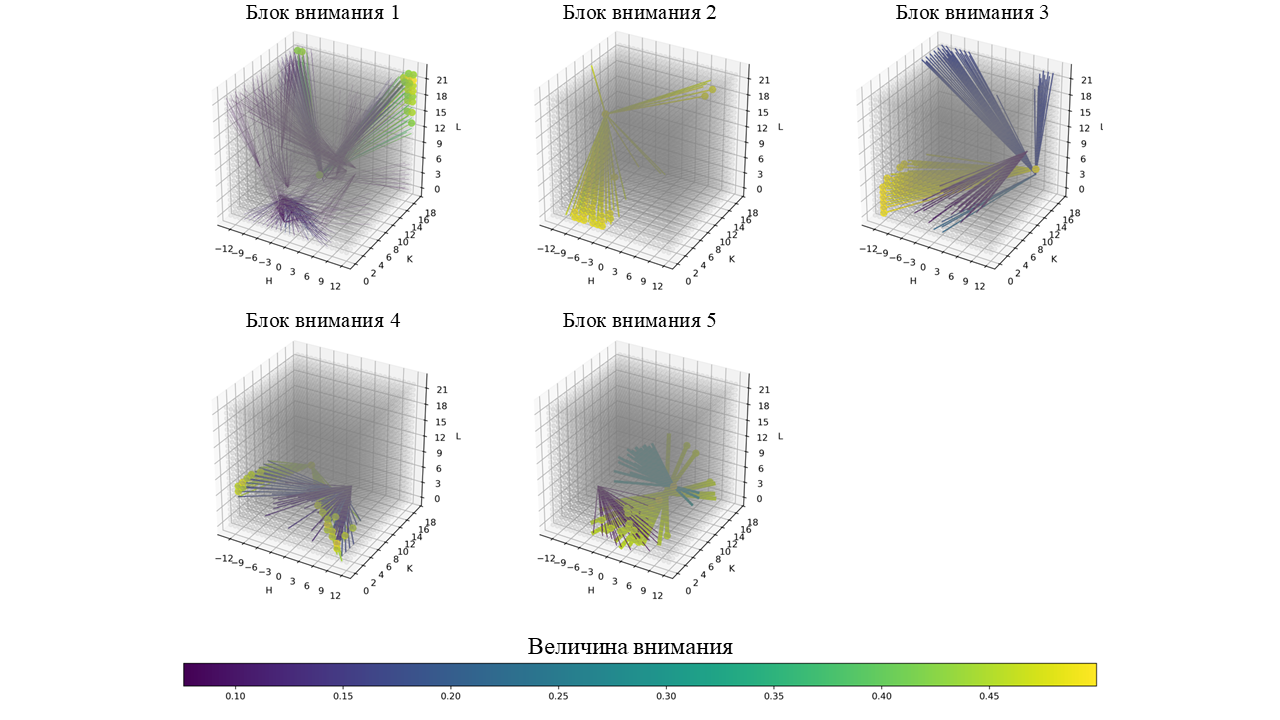
\includegraphics[width=1\textwidth]{figures/attention.png}
    \caption{Связи внимания в блоках трансформера}
    \label{attention_maps}
\end{figure}

Для количественного подтверждения этой гипотезы, было проанализировано распределение значений внимания для наиболее сильных связей в каждом блоке трансформера (рис. \ref{att_hist}). Особый интерес представляет сравнение двух типов связей: между точками, соответствующим систематическим погасаниям и обычными отражениями. Можно заметить, что во время сбора общего контекста в первом блоке распределение значений внимания для связей с погасшими отражениями сопоставимо с таковым для обычных отражений. Это логично, поскольку на этом этапе модель еще не дифференцирует типы отражений, а просто собирает общую информацию о структуре. Однако уже во втором блоке наблюдается значительно уменьшение связей внимания, соединяющих погасания. Это указывает на то, что модель начинает осознавать, что эти отражения несут меньше полезной информации, требуемой для предсказывания дальних отражений. В третьем же блоке модель игнорирует точки обратного пространства, соответствующие систематическим погасаниям, и в выходном тензоре на соответствующих местах стоят нули. 

\begin{figure}[H]
    \centering
    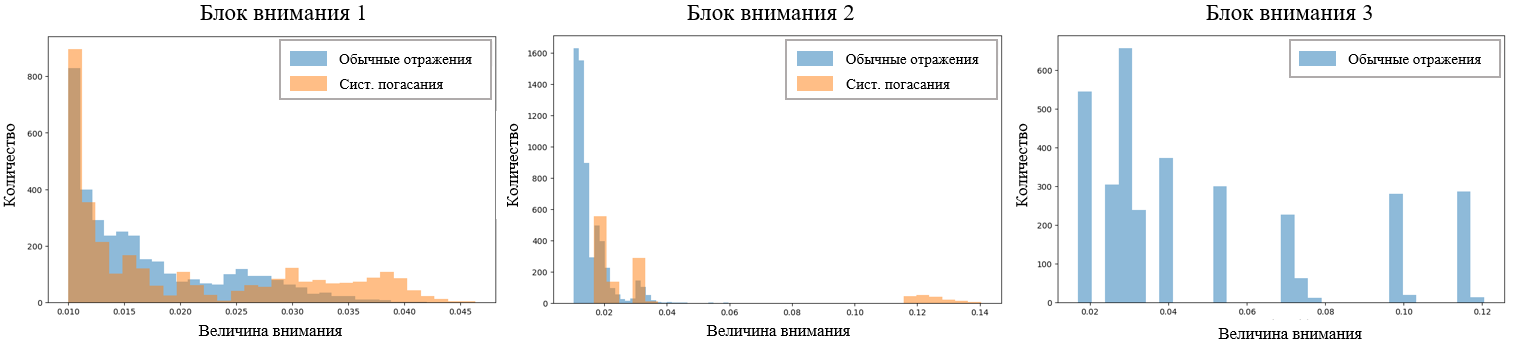
\includegraphics[width=1\textwidth]{figures/attention_hist.png}
    \caption{Распределение величин внимания в первых блоках трансформера.}
    \label{attention_maps}
\end{figure}

Такое поведение модели демонстрирует, что она не просто запомнила шаблоны из обучающей выборки, а научилась автоматически определять и игнорировать отражения, соответствующие систематическим погасаниям (если такие присутствуют). Трансформер действительно успешно выучил кристаллографическую закономерность, значит, данная архитектура может являться ключевой для дальнейших исследований применения методов глубокого обучения для решений кристаллографических задач.

Для понимания внутренней работы моделей на основе UNet, был проведен анализ первого блока обеих архитектур с помощью метода GradCAM (рис. \ref{gradcam}) \cite{selvaraju_grad-cam_2020}. Этот метод позволяет визуализировать, какие области входных данных имеют наибольшее влияние для принятия решений моделью.


\begin{figure}[H]
     \centering
     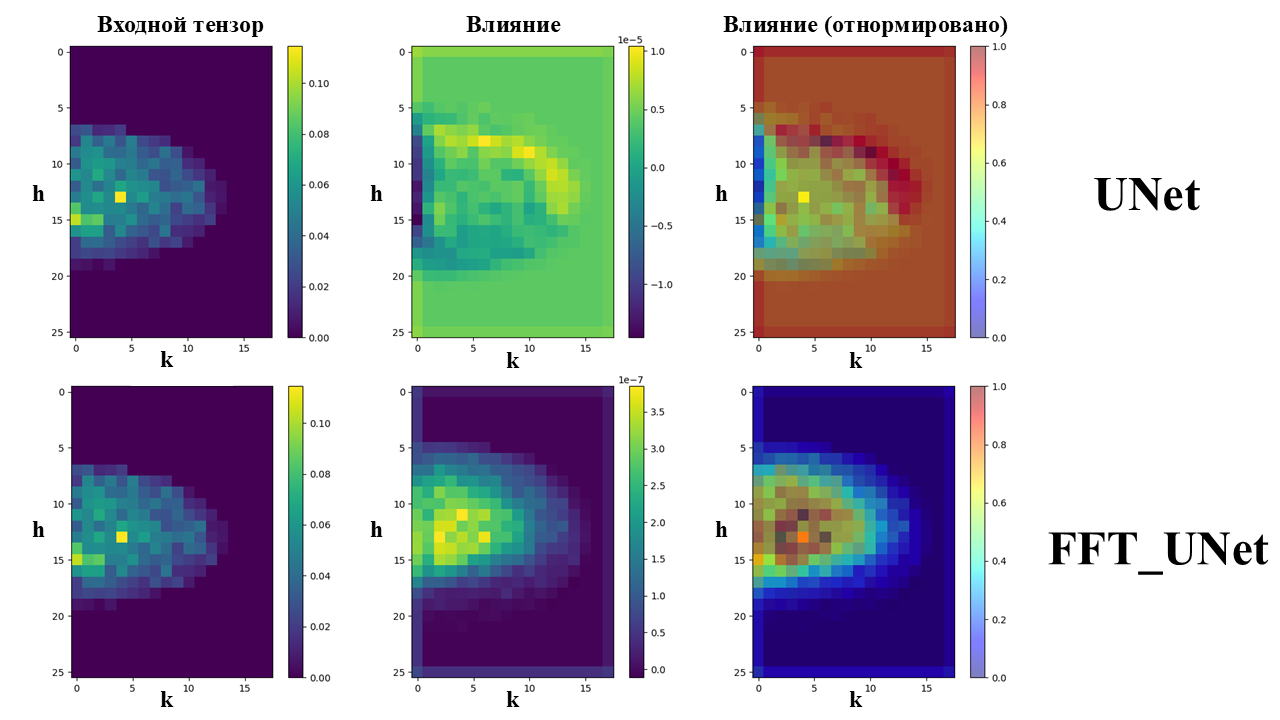
\includegraphics[width=1\textwidth]{figures/attribute_map.png}
     \caption{Тепловые карты влияния GradCAM}
     \label{gradcam}
\end{figure}

%\begin{figure}[H]
%    \centering
%    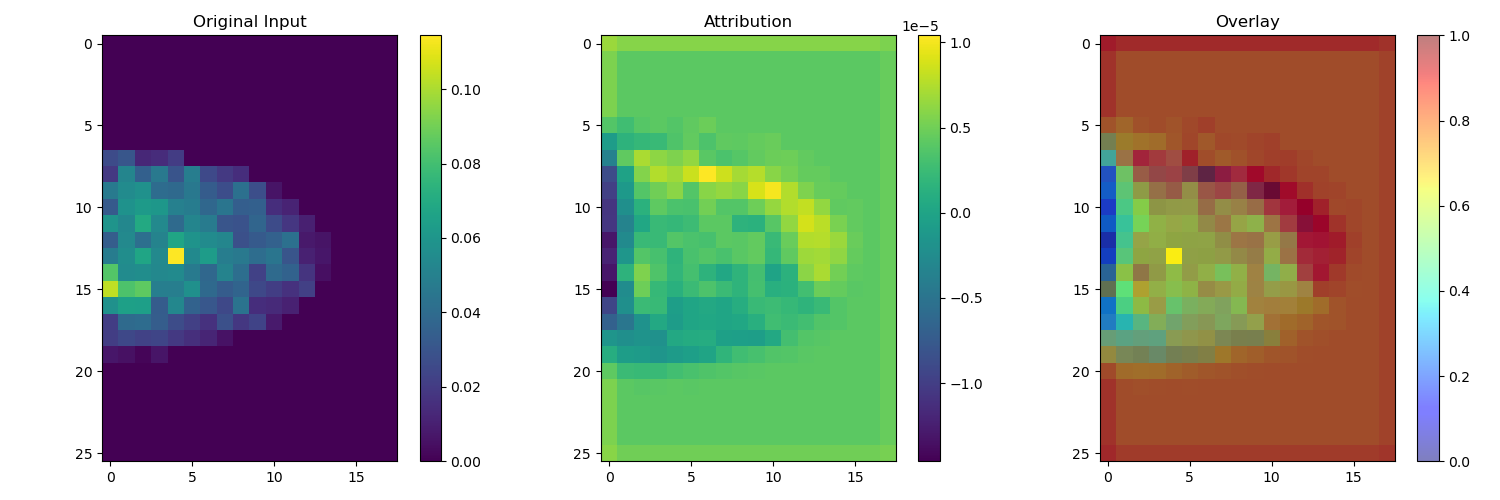
\includegraphics[width=1\textwidth]{figures/attribution_overlay.png}
%    \caption{Анализ первого блока UNet с помощью GradCAM}
%    \label{gradU}
%\end{figure}
%
%\begin{figure}[H]
%    \centering
%    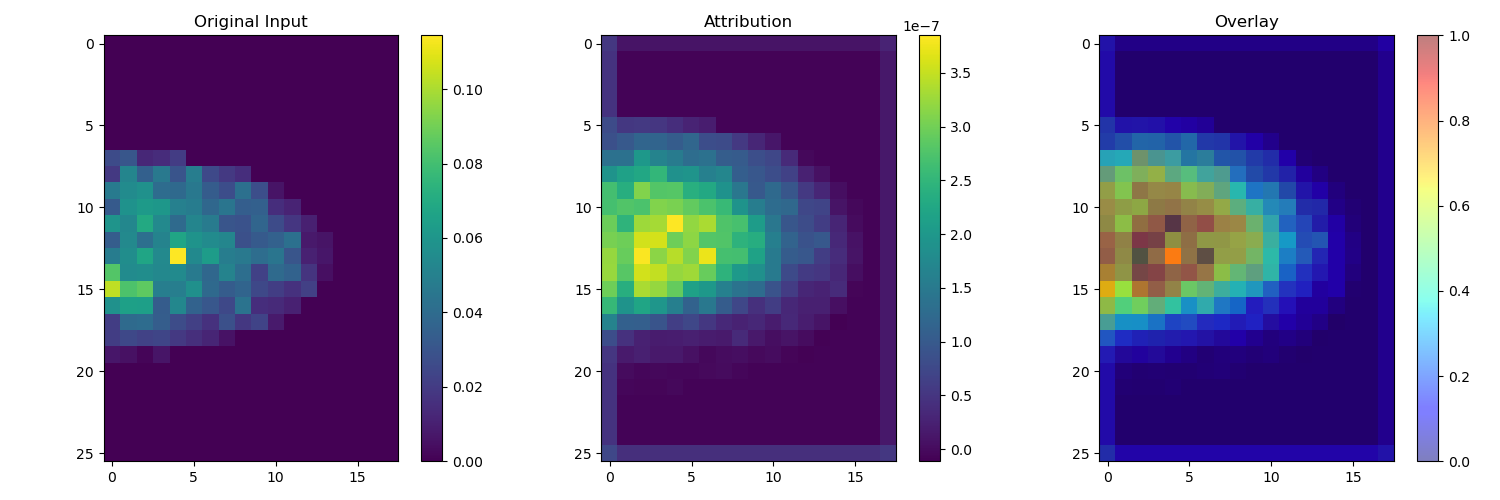
\includegraphics[width=1\textwidth]{figures/attribution_overlay_fft.png}
%    \caption{Анализ первого блока FFT\_UNet с помощью GradCAM}
%    \label{gradFFT}
%\end{figure}

Анализ тепловой карты влияния для модели UNet показал интересную особенность: модель концентрируется во всем пространстве за пределами изначальной дифракционной картины низкого разрешения. Это может указывать на то, что модель UNet не полностью учитывает физические ограничения задачи и пытается извлечь информацию из областей, где она физически не может существовать. 

В отличие от UNet, паттерн внимания для FFT\_UNet выглядит более физически обоснованным. Значения влияния распространяются преимущественно на область входной дифракционной картины и немного выходят за её границы. Это поведение более физически обосновано, так как модель ищет информацию вблизи границ дифракционной картины, где могут находиться важные детали структуры. 

Это различие в поведении моделей может объяснять, почему FFT\_UNet показывает лучшие результаты в восстановлении дифракционной картины. Её способность более точно определять области, где может находиться полезная информация, и игнорировать физически нереалистичные области, делает её более эффективной в поиске правильного решения.



\begin{figure}[H]
    \centering
    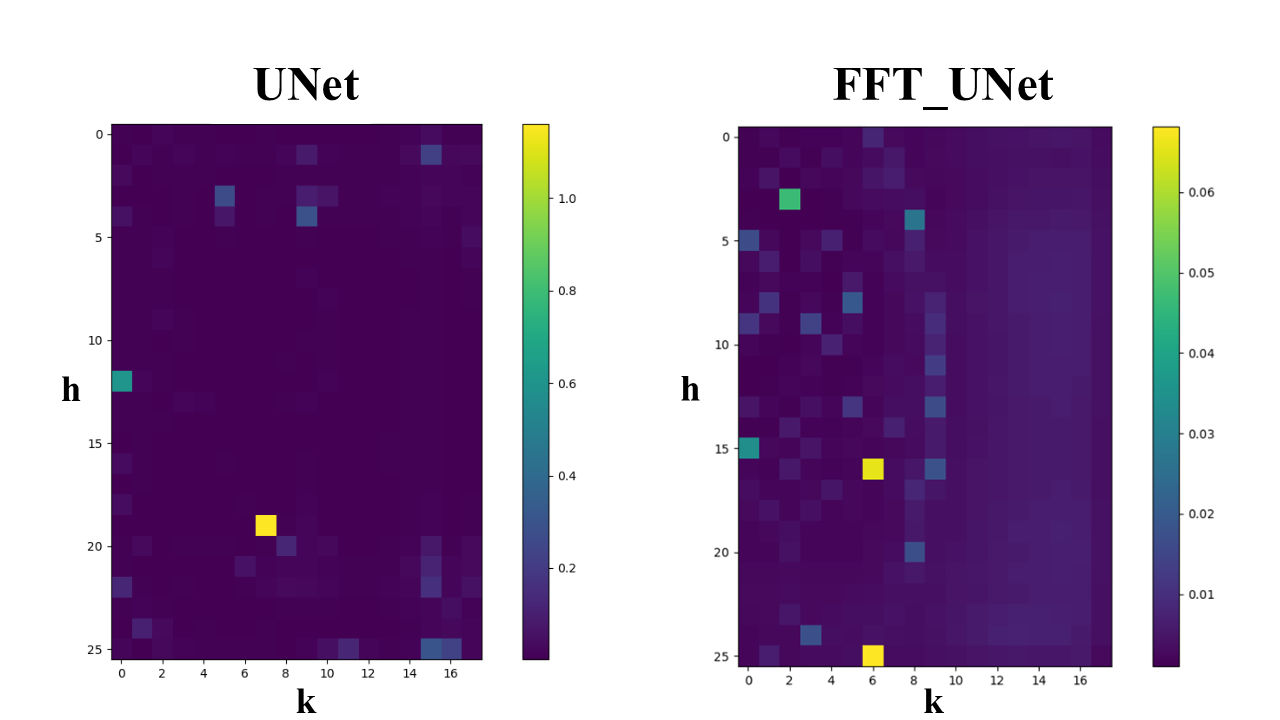
\includegraphics[width=1\textwidth]{figures/sensitivity.png}
    \caption{Тепловые карты чувствительности}
    \label{sens}
\end{figure}


Для оценки устойчивости моделей к шуму в экспериментальных данных был проведен анализ карт чувствительности (рис. \ref{sens}). Карты чувствительности показывают, как сильно меняется выход модели при добавлении случайного шума к входным данным, что позволяет оценить устойчивость модели в различных областях обратного пространства. Базовая модель UNet демонстрирует неустойчивое поведение – выход модели может измениться при добавлении шума на очень большие значения. Модель с Фурье-преобразованием FFT\_UNet стабильно работает при наличии шума в данных. Высокая робастность в большей части пространства указывает на то, что модель научилась извлекать надежные признаки из данных и не переобучилась на конкретные значения амплитуд структурных факторов. 


\subsection{Проверка на реальных данных}

Хотя модели демонстрируют обнадеживающие результаты на реальных моноклинных структурах из Кембриджского Банка Структурных данных, качество восстановления тензора отражений все еще недостаточно для решения структуры с помощью программы SHELXT. На рис. \ref{recon_ex} представлены характерные сечения тензора отражений для реальной структуры, где R-фактор восстановленного тензора с помощью FFT\_UNet составляет 0.35.

\begin{figure}[H]
    \centering
    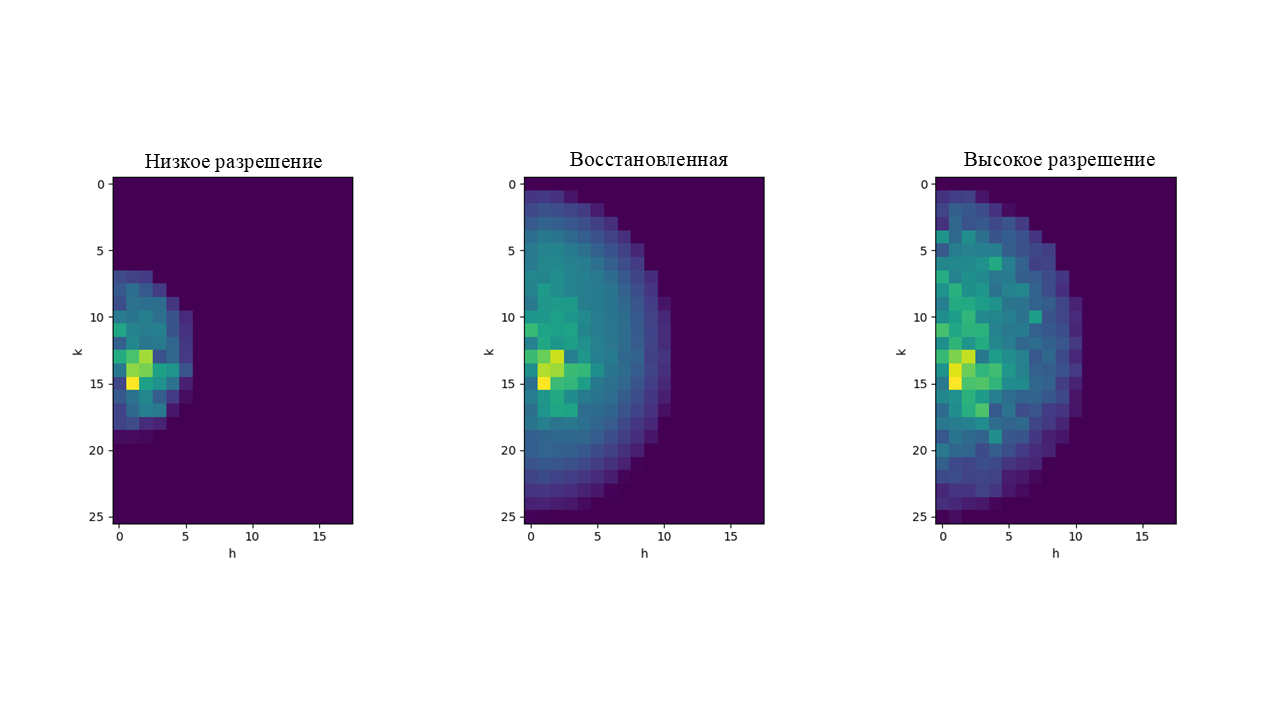
\includegraphics[width=1\textwidth]{figures/real.png}
    \caption{Типичная реконструкция дифракции реальной структуры, $R = 0.346$}
    \label{recon_ex}
\end{figure}

Анализ результатов показывает, что нейронная сеть успешно справляется с определением общих характеристик дифракционной картины. Она точно предсказывает границы дифракционной картины и корректно восстанавливает средние значения амплитуд структурных факторов по небольшим областям. Однако изменения амплитуд между соседними точками обратного пространства недостаточно четко выражены, что приводит к потере важных деталей в распределении амплитуд. 

Это ограничение становится особенно критичным, если учесть фундаментальную особенность дифракционных отражений: каждое отражение содержит информацию о всей кристаллической структуре, и для успешного решения проблемы фаз необходимо чрезвычайно точное определение амплитуды в каждой точке. Хотя модели глубокого обучения выявляют некоторые кристаллографические закономерности, они не достигают необходимой точности в численном определении значений для каждой точки.

Таким образом, методы глубокого обучения демонстрируют значительный потенциал в распознавании кристаллографических закономерностей в обратном пространстве, но сталкиваются с фундаментальным ограничением при решении проблемы фаз. Это ограничение связано с необходимостью чрезвычайно точного численного восстановления амплитуд отражений, что требует более точного подхода к определению значений в каждой точке. Это наблюдение указывает на необходимость разработки новых архитектур или подходов, которые могли бы сочетать способность к распознаванию паттернов с более точным численным восстановлением.

\subsection{Дальнейшие планы и предложения}

Было показано, что методы глубокого обучения успешно схватывают кристаллографические закономерности, однако из-за специфики обратного пространства для решения проблемы фаз им не хватает точности. Совершив переход в прямое пространство, можно предположить, что нейронные сети справятся с поставленной задачей.

Для решения проблемы фаз часто используется функция Паттерсона:

\begin{center}
    $P(u, v, w) = \sum\limits_{h,k,l\in Z} |F(h,k,l)|^2e^{-2\pi i(hu+kv+lw)}$
\end{center}

Функция Паттерсона является Фурье-преобразованием интенсивностей дифракционных максимумов, где за их фазы приняты нули. Таким образом, перейдя от тензора отражений к карте функции Паттерсона - получается классическая задача повышения разрешения изображений, поскольку для дифракционной картины низкого разрешения получится Фурье-образ низкого разрешения, разрешение которого требуется повысить так, чтобы восстановленная картина соответствовала Фурье-образу дифракционной картины высокого разрешения. После увеличения разрешения трехмерной картины функции Паттерсона, мы можем вернуться в обратное пространство, рассчитав интенсивности (и из них амплитуды) рентгенодифракционных отражений, и решить проблему фаз с помощью уже существующих ab initio методов.

\begin{figure}[H]
    \centering
    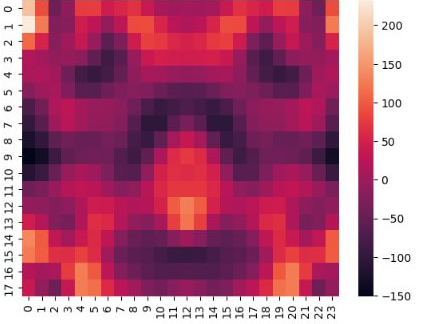
\includegraphics[width=0.5\textwidth]{figures/patt_high.png}\hfill
    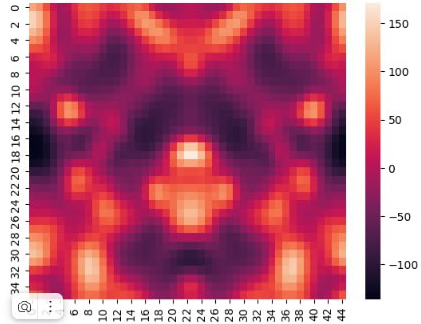
\includegraphics[width=0.5\textwidth]{figures/patt_low.png}
    \caption{Типичное сечение функции Паттерсона по данным низкого (слева) и высокого (справа) разрешения}
    \label{patt}
\end{figure}